%!TEX root = PMP_ClockPendulumAnalyzer.tex
\section{Test}
		\subsection{Testumgebung}
        In diesem Kapitel ist die ganze Testumgebung erläutert, damit exakte und nachvollziehbare Test gemacht werden können.
        \subsubsection{Aufstellung}
        Der Pendulum Analyzer wird mittels einer normalen Wand-Pendeluhr getestet. Dazu wird die Uhr in einer dafür hergestellten Verschalung aufgehängt.
        \begin{figure}[H]
            \centering
            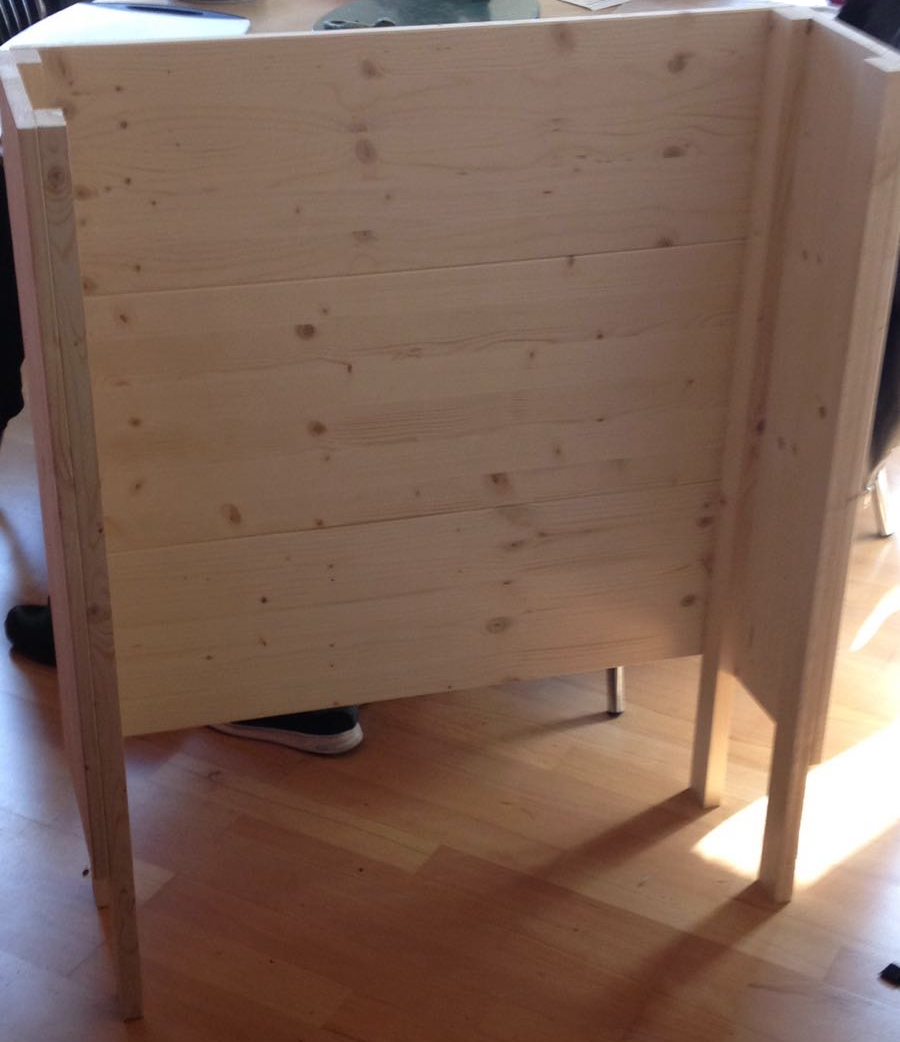
\includegraphics[width=.5\textwidth]{verschalung.png}
            \caption{Verschalung für die Pendeluhr}
        \end{figure}

        \noindent Die Uhr hat eine Fläche auf der das Gerät platziert werden kann. Es wird daher keine zusätzliche Montage für die Sensoren gebaut.
        
        \clearpage
        \subsubsection{Sensor Montage}
        Im Prototyp I wird ein Sensor verwendet. Dieser wird an einer einfachen Holzstange montiert. Die Höhe ist verstellbar über 17 Positionen und in der Länge stufenlos.
        \begin{figure}[H]
            \centering
            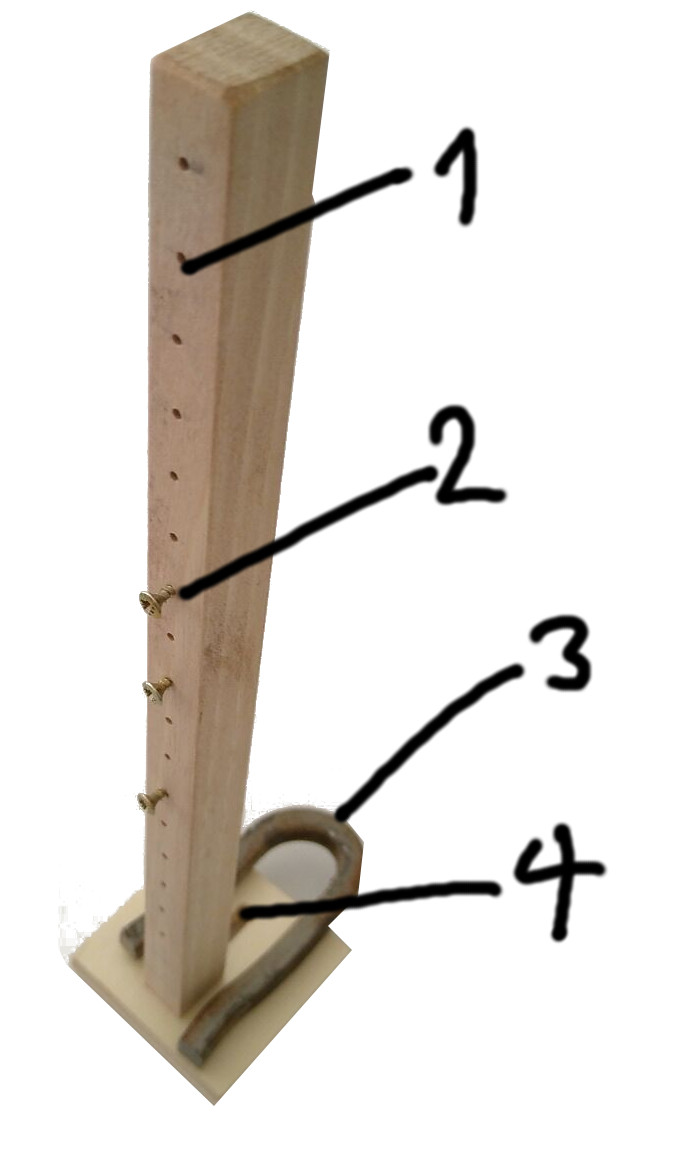
\includegraphics[width=.2\textwidth]{sensoraufhangung.png}
            \caption{Verschalung für die Pendeluhr}
        \end{figure}
        \begin{enumerate}
            \item Loch für die Montage eines Sensorboard
            \item Schraube zum montieren
            \item Gewicht zur Stabilisierung
            \item Langloch zur Feinjustierung der Länge
        \end{enumerate}
        \subsubsection{Software Komponenten}

		\subsection{Testfälle}
			\textit{Was wird durch das Testen abgedeckt}
			\subsubsection{Unit Tests}
			\subsubsection{Blackbox Tests}